\documentclass[a4paper]{article}

\usepackage[utf8]{inputenc}
\usepackage[T1]{fontenc}
\usepackage{textcomp}
\usepackage[english]{babel}
\usepackage{amsmath, amssymb, caption, titlesec, fullpage, multicol, bm, graphicx}
\graphicspath{ {images/} }
\captionsetup{labelformat=empty,labelsep=none}
\newcommand{\sectionbreak}{\clearpage}
\title{Databases labs}
\author{Andrii Stadnik}

\begin{document}
\maketitle
\tableofcontents
\section{Lab 1}
\subsection{}
\begin{align*}
    S &= \{name, salary, city\} \\
    r &=
    \begin{aligned}[t]
            &\{(Andrii, 2500, Kyiv), \\
            &(Jonathan, 1200, San-Diego), \\
            &(Potato, 4500, Potato-city)\}
    \end{aligned} \\
    EMP &= (S, r)
.\end{align*}
\subsection{}
\[
    *_{city}(EMP_1) = Kyiv
.\]
\subsection{}
\[
    EMP_1 \overline{\cup} EMP_1 = EMP_1
.\]
\subsection{}
\[
    a \implies R(S, r) = R(\{a \implies \hat{S}, \forall \hat{S} \in S\}, (a \implies
    \hat{r}, \forall \hat{r} \in r))
.\]
\section{Lab 2}
\subsection{}
\begin{flalign*}
    \begin{aligned}
        FILTER(S^2(<>, *_{a}, *_{b})) &\big((a, b), \{(a: 1, b: 2), (a: 3, b: 3)\}\big) \\
                                      &= \big( (a, b), \{(a: 1, b: 2)\} \big)
    \end{aligned} \\
    \begin{aligned}
        S^{2}(SEL(a = *_{a}), FILTER(S^{2}(<, *_{b}, *_{c}))) &\big((a, b, c), \{(a: b, b: 2, c: 3)\}\big) \\
                                                              &= \big((a), \{(a: 3)\}) \\
    \end{aligned} \\
    \begin{aligned}
        S^1(FILTER(S^2(<, *_{b}, *_{c})), *_{t}) &\Big((t), {(t: \big((b, c), \{(b: 1, c: 2), (b: 3, c: 3)\}\big))}\Big) \\
                                                 &= \big((b, c), \{(b: 1, c: 2)\}\big)
    \end{aligned} \\
.\end{flalign*}



\subsection{}
\begin{itemize}
    \item SELECT * FROM t WHERE t.b < t.c;
    \item SELECT x.*, y.* FROM t1 x CROSS JOIN t2 y;
    \item SELECT x.c - 11 AS a, y.d AS b FROM t1 x CROSS JOIN t2 y;
\end{itemize}
\subsection{}
\begin{itemize}
    \item FILTER(=, *a, 5)( $t_1$ )
    \item SEL($a_1$ = *a, $b_1$ = *b + 7)($t_1$)
    \item $S^1$(SEL($a_1$ = *$t_1$.a, $b_1$ = *$t_1$.b, $x_1$ = $t_2$.x),
        $S^2$(FILTER($S^2$(=, *$t_1$.a, *$t_2$.a), $S^1$ ($CJ_{t_1, t_2}$, $*_{t_1}$, $*_{t_2}$ ))))
\end{itemize}
\subsection{}
\[
    R_1(S, r_1) \overline{\cup} R_2(S, r_2) = \hat{R}(S, r_1 \overline{\cup} r_2)
.\]
\section{Lab 3}
\subsection{}
\begin{table}[htpb]
    \centering
    \caption{Relation}
    \begin{tabular}{|c|c|c|}
        \hline
        X & Y & Z \\
        \hline\hline
        $x_1$ & $y_1$ & $z_1$ \\
        \hline
        $x_1$ & $y_1$ & $z_2$ \\
        \hline
        $x_2$ & $y_1$ & $z_1$ \\
        \hline
        $x_2$ & $y_1$ & $z_3$ \\
        \hline
    \end{tabular}
\end{table}
Functional depends:
% \begin{multicols}{3}
\begin{itemize}
    \itemsep -0.5em
    \item $ X \to X$
    \item $ X \to Y$
    \item $ Z \to Z$
    \item $ Z \to Y$
    \item $ Y \to Y$
    \item $ XZ \to Y$
\end{itemize}
\begin{table}[htpb]
    \centering
    \caption{Relation}
    \begin{tabular}{|c|c|c|}
        \hline
        X & Y & Z \\
        \hline\hline
        $x_1$ & $y_1$ & $z_1$ \\
        \hline
        $x_1$ & $y_1$ & $z_2$ \\
        \hline
        $x_2$ & $y_1$ & $z_1$ \\
        \hline
        $x_2$ & $y_1$ & \boldsymbol{$z_2$} \\
        \hline
    \end{tabular}
\end{table}
Functional depends:
% \begin{multicols}{3}
\begin{itemize}
    \itemsep -0.5em
    \item $ X \to X$
    \item $ X \to Y$
    \item $ Z \to Z$
    \item $ Z \to Y$
    \item $ Y \to Y$
    \item $ XZ \to Y$
\end{itemize}
% \end{multicols}
\subsection{}
SELECT * FROM R r1, R r2 WHERE r1.A=r2.A AND r1.B <> r2.B

This query will output an empty set if functional dependency holds
\subsection{}
SELECT * FROM R r1, R r2 WHERE (r1.A=r2.A AND r1.B=r2.B) AND (r1.E <> r2.E OR
r1.D <> r1.D)

This query will output an empty set if functional dependency holds
\subsection{}
The program and the sample inputs are in the labs folder
\section{Lab 4}
\subsection{}
Remove column C from the main relation, and create another one with columns B
and C
\subsection{}
Each value from A is related to one and only one value from B.
\subsection{}
Prove that ACD, BCD and CDE are the keys
\begin{itemize}
    \item \begin{flalign*}
            ACD &\to ACD (reflexivity) &\\
            A   &\to B &\\
            ACD &\to B (augmentation) &\\
            ACD &\to ABCD (additivity) &\\
            BC  &\to E &\\
            ACD &\to BC (decomposition) &\\
            ACD &\to E (transitivity) &\\
            ACD &\to ABCDE (additivity) &\\
        \end{flalign*}
    \item \begin{flalign*}
            BCD &\to BCD (reflexivity) &\\
            BC  &\to E &\\
            BCD &\to E (augmentation) &\\
            BCD &\to BCDE (additivity) &\\
            ED  &\to A &\\
            BCD &\to ED (decomposition) &\\
            BCD &\to A (transitivity) &\\
            BCD &\to ABCDE (additivity) &\\
        \end{flalign*}
    \item \begin{flalign*}
            CDE &\to CDE (reflexivity) &\\
            ED  &\to A &\\
            CDE &\to ED (decomposition) &\\
            CDE &\to A (trainsitivity) &\\
            CDE &\to ACDE (additivity) &\\
            A   &\to B &\\
            CDE &\to A (decomposition) &\\
            CDE &\to B (transitivity) &\\
            CDE &\to ABCDE (additivity)
        \end{flalign*}
\end{itemize}
Prove that ABCD, ACDE and BCDE are superkeys
\begin{itemize}
    \item \begin{flalign*}
            ABCD &\to ABCDE &\\
            A &\to B &\\
            AACD &\to ABCD (pseudotransitivity)
        \end{flalign*}
    \item \begin{flalign*}
            ACDE &\to ABCDE &\\
            ED &\to A
            EDCDE &\to ABCD (pseudotransitivity)
        \end{flalign*}
    \item \begin{flalign*}
            BCDE &\to ABCDE &\\
            ED &\to A &\\
            A &\to B &\\
            ED &\to B (transitivity) &\\
            EDCED &\to ABCDE
        \end{flalign*} (Cause of the transitivity rule it's sufficient to only add
        ED and not add B)
\end{itemize}
\subsection{}
The program and the sample inputs are in the labs folder
\section{Lab 5}
\subsection{}
Key is $ACE$, so we have 3 relations: $ACE \to ABCDE$, $A \to B$ and $C \to D$.
Let's first divide it by the second relation $A \to B$ :
\begin{itemize}
    \item $ACDE$ with relations $C \to D$, $ACE \to ACDE$
    \item $AB$ with relation $A \to B$
\end{itemize}

Now we have to get rid of the $C \to D$ relation, so we divide it once again by it, and get three relations:
\begin{itemize}
    \item $ACE$ with relation $ACE \to ACE$
    \item $CD$ with relation $C \to D$
    \item $AB$ with relation $A \to B$
\end{itemize}
\subsection{}
Key is $ACB \to ABCEF$, so we again have 3 relations: $ACB \to ABCEF$, $AC \to
E$, $B \to F$. Let's start with the 2nd relation:
\begin{itemize}
    \item $ACBF$ with relations $ACB \to ACBF$, $B \to F$
    \item $ACE$ with relation $AC \to E$
\end{itemize}
Now we have to get rid of the $B \to F$ relation, so we divide it once again by it, and get three relations:
\begin{itemize}
    \item $ACB$ with relations $ACB \to ACBF$
    \item $ACE$ with relation $AC \to E$
    \item $BF$ with relation $B \to F$
\end{itemize}
\subsection{}
Key is $BDEF \to ABCDEF$, so we have 3 relations: $BDEF \to ABCDEF$, $B \to
C$, $D \to A$. Let's start with the 2nd relation:
\begin{itemize}
    \item $ABDEF$ with relations $BDEF \to ABDEF$, $D \to A$
    \item $BC$ with relation $B \to C$
\end{itemize}
Now we have to get rid of the $D \to A$ relation, so we divide it once again by it, and get three relations:
\begin{itemize}
    \item $BDEF$ with relations $BDEF \to BDEF$
    \item $BC$ with relation $B \to C$
    \item $DA$ with relation $D \to A$
\end{itemize}
\subsection{}
The program and the sample inputs are in the labs folder
\section{Lab 6}
\subsection{}
\begin{enumerate}
    \item $AB \to C$
    \item $AC \to B$
    \item $B \to D$
    \item $BC \to A$
    \item $AC \to C $
\end{enumerate}
We can remove the last one:
\begin{itemize}
    \item $C \to C$ (reflexivity)
    \item $C \subset AC \implies AC \to C$, which means that we can derive the 5th equation, and so we can remove it
\end{itemize}
\subsection{}
% Key is $B$. If we divide the relation into 3 relations:  $BC$, $CD$ and $CA$, this schema will be in 3NF.
Key is $B$. It has the transitive dependencies $C \to D$ and $C \to A$, so we have to divide the relation into 2: $BC$ and $CDA$.
\subsection{}
Key is $A$. If we divide the relation into 2 relations: $ACB$ and $BCD$, it will be in the 3NF.% If we add one more relation $ACB$, it will be in the 3NF. Though we could split it only in 2 relations: $ACB$ and $BCD$, and all functional dependencies will hold.
\subsection{}
Key is $A$. We can prove that $A \to C$: since $A \to DE$, $A \to D$, and since $A \to D$ and $D \to B$, $A \to B$ (transitivity). And since $AB \to C$ and $A \to B$, $A \to C$. We have to divide it into $ADEC$ and $DB$.
\section{Lab 7}
\subsection{}
\begin{figure}[htpb]
    \centering
    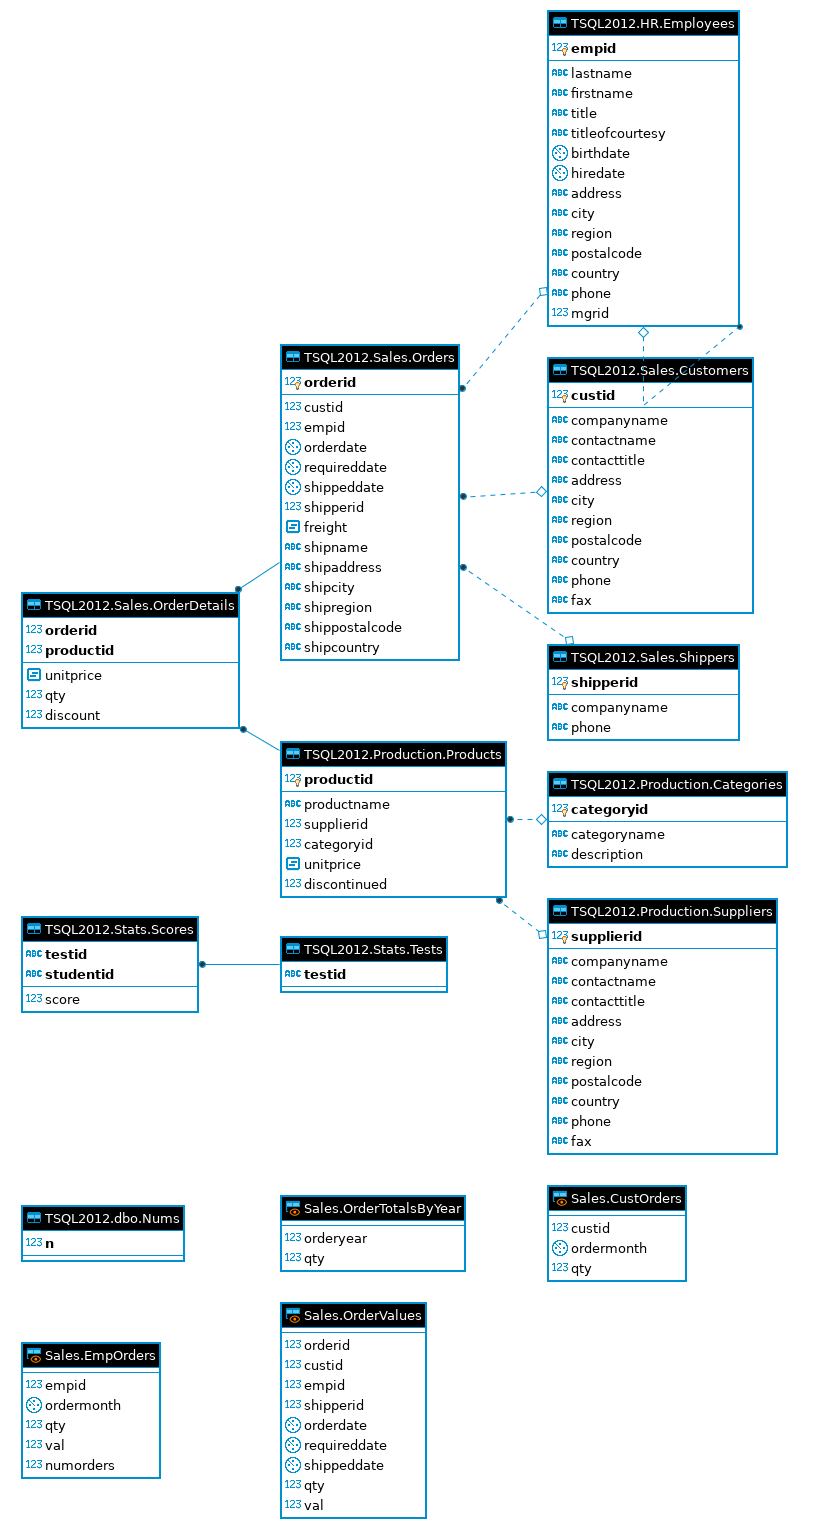
\includegraphics[width=0.6\textwidth]{er_diagram}
    \caption{er\_diagram}
    \label{fig:er_diagram}
\end{figure}
\clearpage
On this image we can clearly see all connections. There are a couple types of connections
\begin{itemize}
    \item One to many:
        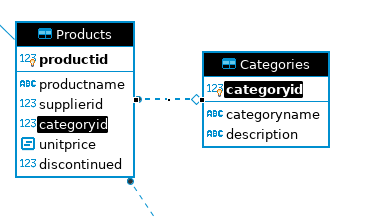
\includegraphics[width=0.3\textwidth]{one_to_many}
    \item One to one:
        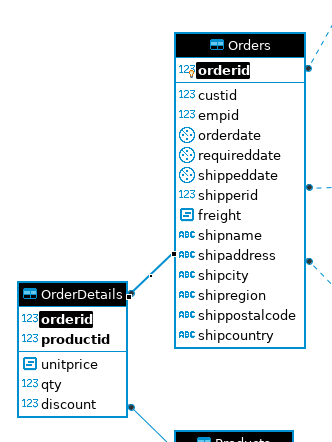
\includegraphics[width=0.3\textwidth]{one_to_one}
    \item Connection to itself:
        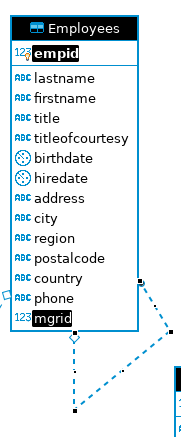
\includegraphics[width=0.3\textwidth]{connection_to_itself}
\end{itemize}
Also there are a couple of weak entities (an entity is called weak if it's primary
key is a superset of the primary key of the related entity):
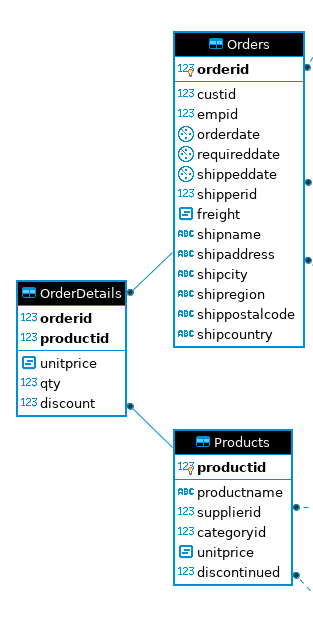
\includegraphics[width=0.3\textwidth]{weak_connection}
\end{document}

vim:set et sw=4 ts=4 tw=0:
